\documentclass[10pt]{article}

\usepackage{hyperref}

%Math
\usepackage{amsmath}
\usepackage{amsfonts}
\usepackage{amssymb}
\usepackage{amsthm}
\usepackage{ulem}
\usepackage{stmaryrd} %f\UTF{00FC}r Blitz!

%PageStyle
\usepackage[ngerman]{babel} % deutsche Silbentrennung
\usepackage[utf8]{inputenc} 
\usepackage{fancyhdr, graphicx}
\usepackage[scaled=0.92]{helvet}
\usepackage{enumitem}
\usepackage{parskip}
\usepackage[a4paper,top=2cm]{geometry}
\setlength{\textwidth}{17cm}
\setlength{\oddsidemargin}{-0.5cm}


% Shortcommands
\newcommand{\Bold}[1]{\textbf{#1}} %Boldface
\newcommand{\Kursiv}[1]{\textit{#1}} %Italic
\newcommand{\T}[1]{\text{#1}} %Textmode
\newcommand{\Nicht}[1]{\T{\sout{$ #1 $}}} %Streicht Shit durch

%Arrows
\newcommand{\lra}{\leftrightarrow} 
\newcommand{\ra}{\rightarrow}
\newcommand{\la}{\leftarrow}
\newcommand{\lral}{\longleftrightarrow}
\newcommand{\ral}{\longrightarrow}
\newcommand{\lal}{\longleftarrow}
\newcommand{\Lra}{\Leftrightarrow}
\newcommand{\Ra}{\Rightarrow}
\newcommand{\La}{\Leftarrow}
\newcommand{\Lral}{\Longleftrightarrow}
\newcommand{\Ral}{\Longrightarrow}
\newcommand{\Lal}{\Longleftarrow}

% Code listenings
\usepackage{color}
\usepackage{xcolor}
\usepackage{listings}
\usepackage{caption}
\DeclareCaptionFont{white}{\color{white}}
\DeclareCaptionFormat{listing}{\colorbox{gray}{\parbox{\textwidth}{#1#2#3}}}
\captionsetup[lstlisting]{format=listing,labelfont=white,textfont=white}
\lstdefinestyle{JavaStyle}{
 language=Java,
 basicstyle=\footnotesize\ttfamily, % Standardschrift
 numbers=left,               % Ort der Zeilennummern
 numberstyle=\tiny,          % Stil der Zeilennummern
 stepnumber=5,              % Abstand zwischen den Zeilennummern
 numbersep=5pt,              % Abstand der Nummern zum Text
 tabsize=2,                  % Groesse von Tabs
 extendedchars=true,         %
 breaklines=true,            % Zeilen werden Umgebrochen
 frame=b,         
 %commentstyle=\itshape\color{LightLime}, Was isch das? O_o
 %keywordstyle=\bfseries\color{DarkPurple}, und das O_o
 basicstyle=\footnotesize\ttfamily,
 stringstyle=\color[RGB]{42,0,255}\ttfamily, % Farbe der String
 keywordstyle=\color[RGB]{127,0,85}\ttfamily, % Farbe der Keywords
 commentstyle=\color[RGB]{63,127,95}\ttfamily, % Farbe des Kommentars
 showspaces=false,           % Leerzeichen anzeigen ?
 showtabs=false,             % Tabs anzeigen ?
 xleftmargin=17pt,
 framexleftmargin=17pt,
 framexrightmargin=5pt,
 framexbottommargin=4pt,
 showstringspaces=false      % Leerzeichen in Strings anzeigen ?        
}

%Config
\renewcommand{\headrulewidth}{0pt}
\setlength{\headheight}{15.2pt}

%Metadata
\fancyfoot[C]{If you use this documentation for a exam, you should offer a beer to the authors!}
\title{
	\vspace{5cm}
	UTF-8 Vorlage
}
\author{Jan Fässler}
\date{3. Semester (HS 2012)}


% hier beginnt das Dokument
\begin{document}

% Titelbild
\maketitle
\thispagestyle{fancy}

\newpage

% Inhaltsverzeichnis
\pagenumbering{Roman}
\tableofcontents	  	


\newpage
\setcounter{page}{1}
\pagenumbering{arabic}

% Inhalt Start

\section{Problemstellung}

%fokus auf die texterkennung

\subsection{Annahmen}
Der Benutzer kooperiert, er wird nicht versuchen 

\section{Analyse der Problemstellung}

\subsection{Analyse der Visitenkarten}
%Unterschiedliche Farben.
%unterschiedliche fonts

\subsection{Analyse der Handybilder}
Ein Typisches Problem
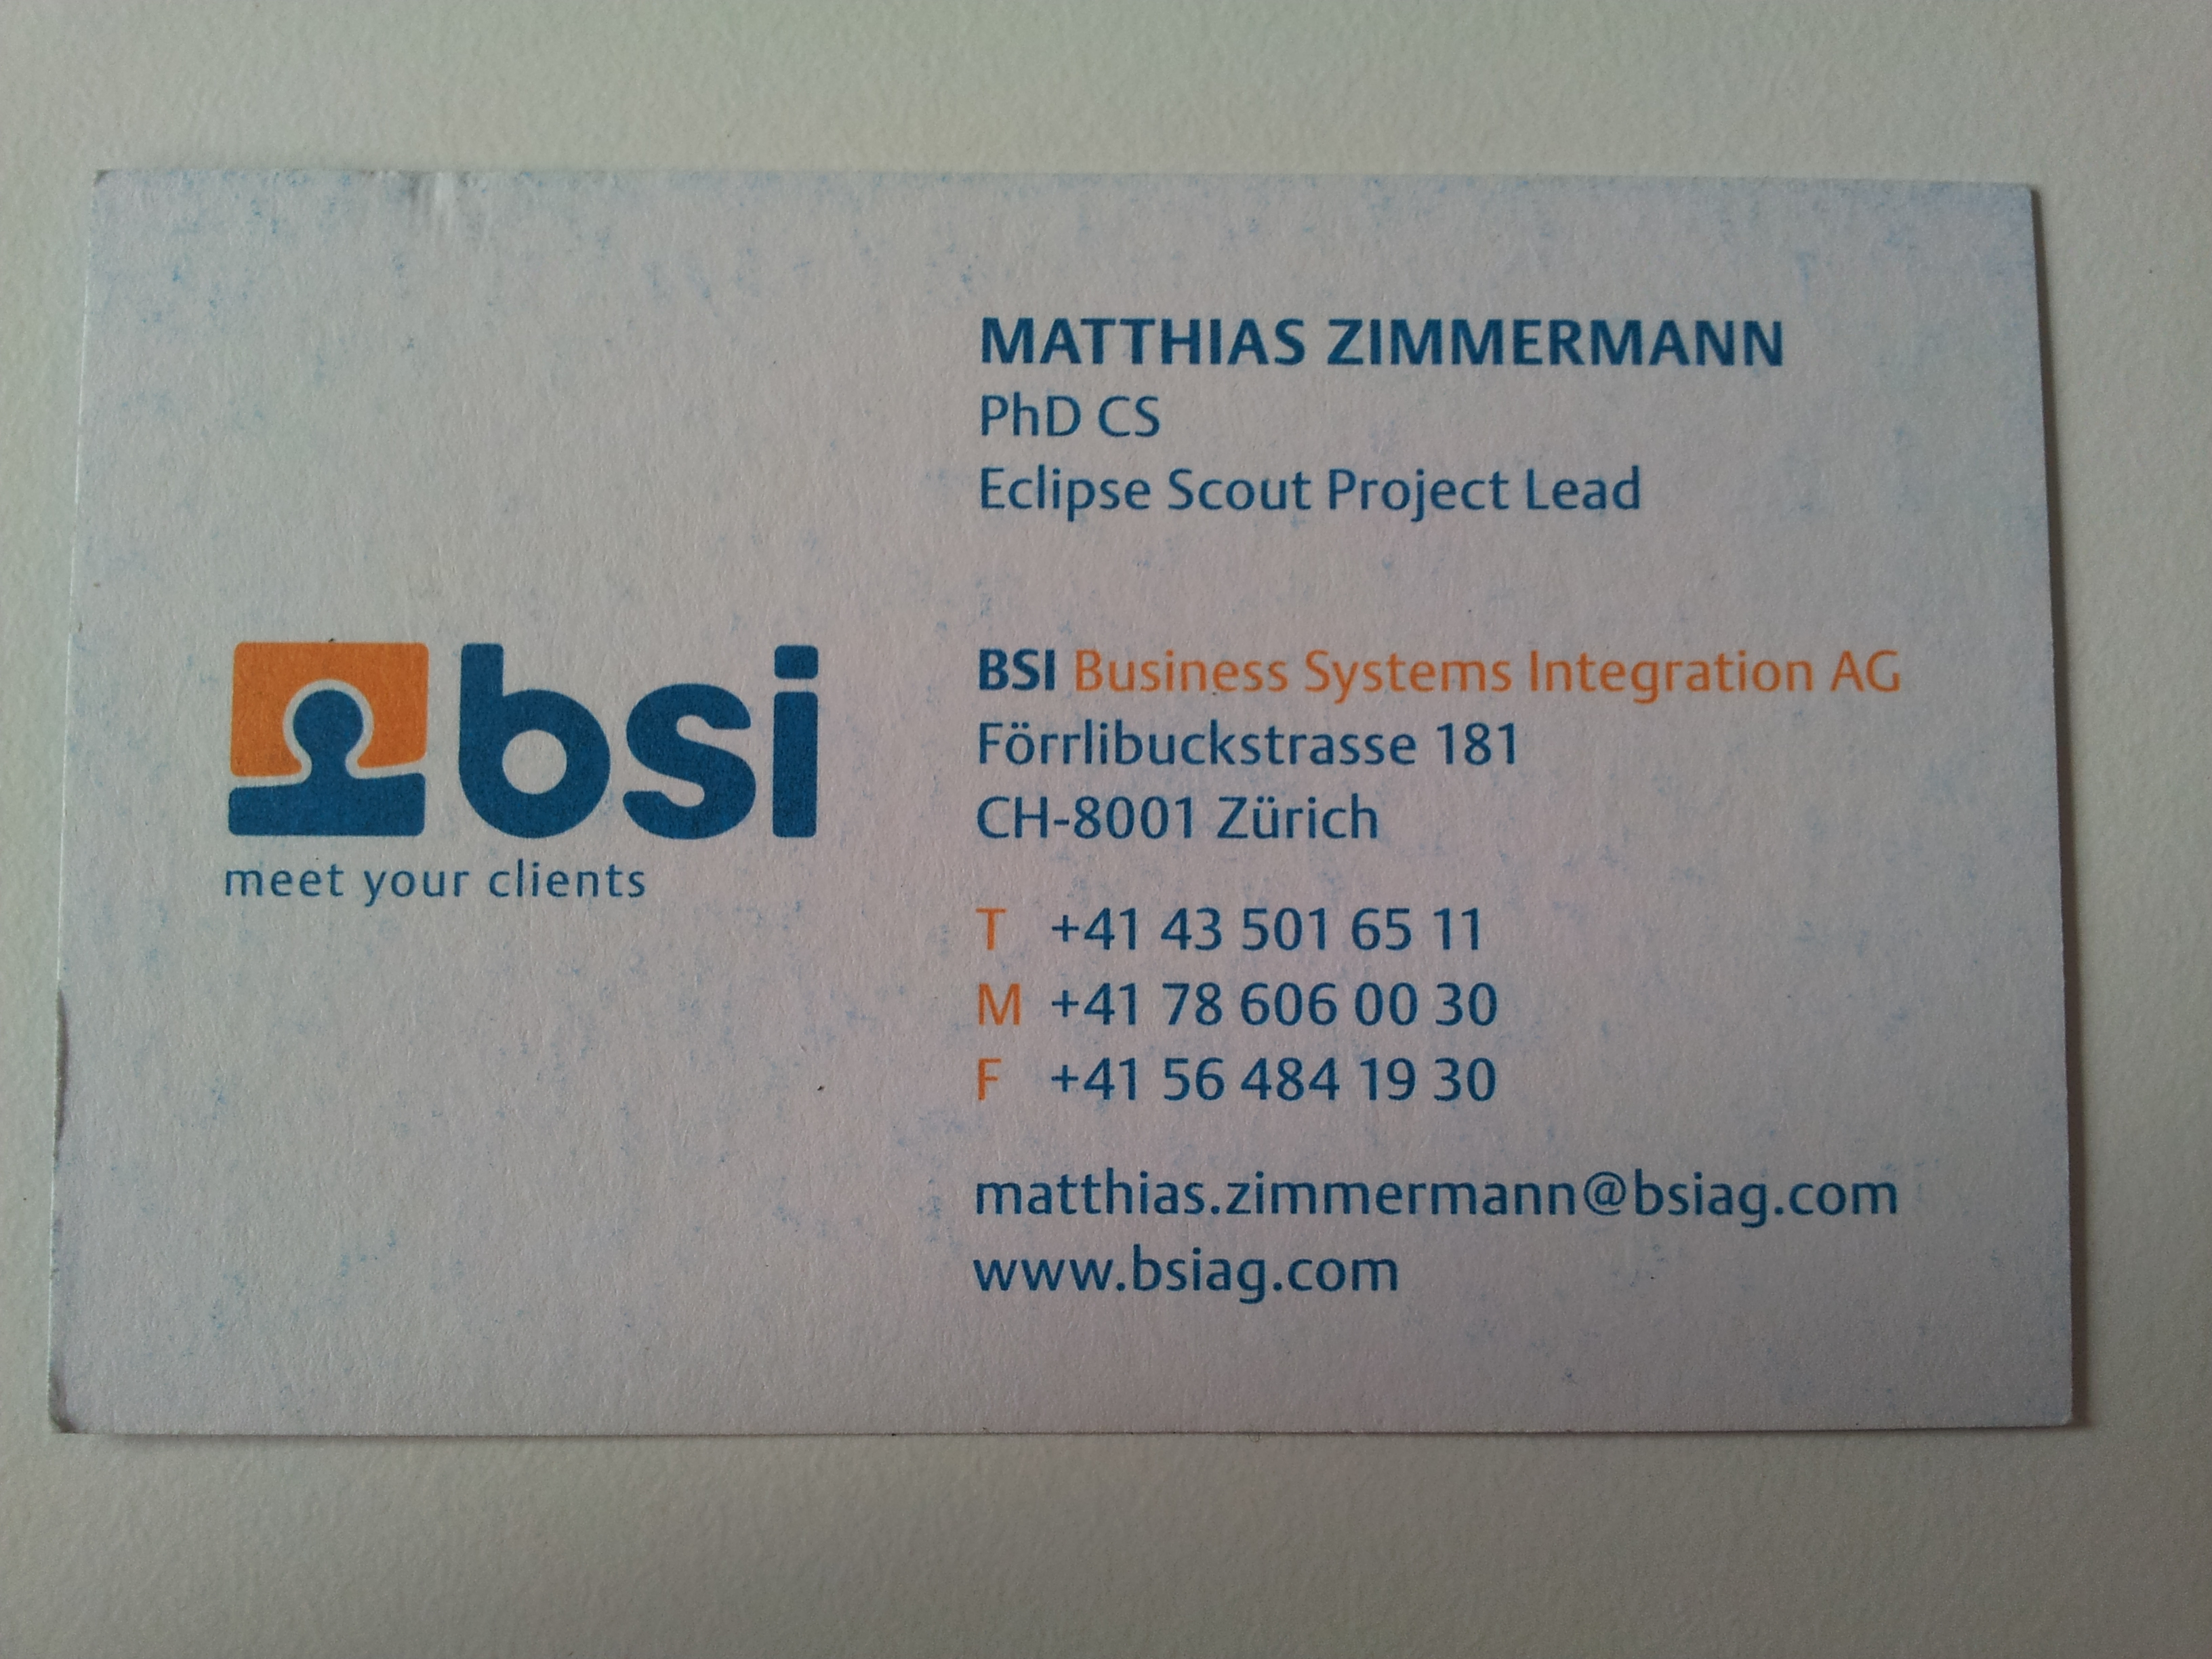
\includegraphics[scale= 0.05]{MZimmermann.jpg}


\section{Testumgebung und Testdaten}
%Müend mer luut Gruntz ha. 

Die Grundidee ist, die Visitenkarten mit dem Cardscanner einzulesen und dessen OCR Output als Solldaten zu verwenden. 

Für die Texterkennung haben wir eine zusätzliche Testumgebung erstellt. So können wir genaue Aussagen über die Qualität der Texterkennung machen und es vereinfacht das Isolieren eines Erkennungsproblems. Diese Umgebung ist unter \ref{tessTestUmgebung} beschrieben.
 
Als Metrik wurde F-Measure eingesetzt. 

\subsection{Visitenkarten Testumgebung}
%Ordnerstruktur

\subsubsection{Vergleich Tesseract-Output mit Cardscan}

\subsubsection{Scale und Offset}
%unser cooles gebastel

\subsection{Tesseract Testumgebung}\label{tessTestUmgebung}
Die zusätzliche Testumgebung ist vergleichsweise Trivial. Auf den Testbildern ist immer der selbe Text zu sehen. Tesseract verarbeitet die Bilder und der erkannte Text wird per String-Diff\footnote{\url{http://code.google.com/p/google-diff-match-patch/}} mit dem Originaltext verglichen.

Der Text hat eine Höhe von ca 30 Pixel, somit hat es in etwa die selbe Auflösung, wie ein klein geschriebener Text auf unseren Visitenkarten-Testbilder.
Wir haben versucht, möglichst weitverbreitete Schriftarten zu verwenden. Dazu haben wir von Webseiten die beliebtesten und meist gehassten Schriftarten genommen\footnote{Quelle: \url{absolutegraphix.co.uk/bestworstfonts.asp?strID=Guest}}. Extrem ausgefallene wie $Bush Script$ Schriftarten wurden nicht miteinbezogen.
Zusätzlich haben wir Schriftarten hinzugefügt, die speziell für Visitenkarten empfohlen werden\footnote{Quelle:\url{ www.psprint.com/resources/powerful-business-card-fonts/}}. Folgende Schriftarten haben wir im Test berücksichtigt:
\begin{itemize}
\item Agency FB
\item Arial
\item Baskerville Old Face
\item Berlin Sans
\item Calibri
\item Century Gothic
\item Elephant
\item Eras Bold
\item Franklin Gothic
\item Garamond
\item Gill Sans
\item Impact
\item Rockwell
\item Tahoma
\item Times New Roman
\item Verdana
\end{itemize}

Die Ausgabe eines Tests sind zwei CSV Dateien. Eine enthält die Precision, Recall, F-Measure, eine Liste der fehlenden Textstellen und eine Liste der Textstellen, welche nicht im Original vorkommen.
Die zweite Datei beinhaltet in wievielen Prozent aller Bilder ein Buchstabe fallsch erkannt wurde. Buchstaben, welche nie fallsch erkannt werden nicht aufgeführt.

\section{Optimierungen}
%titel esch schrott

\subsection{Optimierung Texterkennung}

\subsection{Optimierung Präprozessierung}
%STATISTIKEN


\section{Konfigurationen??????}
%weder en schrott titel

\section{Fazit}

\subsection{Anforderungen an die Kamera}
Für eine annehmbare Texterkennung müssen die Buchstaben eine Höhe von mindestens zehn Pixel haben. Das heisst, die Kamera muss eine genügend hohe Auflösung haben. Die Kamera des $Samsung Galaxy S2$ hat eine Auflösung von 8 Megapixel, das führt dazu dass die Buchstaben der Testbilder eine Höhe von 30 bis 60 Pixel haben. Diese Anforderung wird von einem Smartphone erfüllt, welches 2011 erschien. Die Smartphones, welche heute verkauft werden haben mindestens die selbe Auflösung wie das $Galaxy S2$. Durch die Abonementregelung von Swisscom, Orange und Sunrise wechseln die meisten Smartphone Benutzer alle zwei Jahre auf ein aktuelles Gerät. Somit ist heute kaum mehr ein Smartphone im Betrieb, welches diese Anforderung nicht erfüllt.

Damit der Phansalkar-Algorithmus eine gute Binarisierung durchführen kann, sollte das Bild harte Kanten haben. Wenn die Kamera ein scharfes Bild schiesst, kann der Algorithmus eine gute Binarisierung durchführen.
\begin{figure}[h!]
	\centering
	
\includegraphics[scale= 0.06]{AMathur.jpg}
	
\includegraphics[scale= 0.06]{AMathurPhansalkar.png}
\caption{Beispiel eines scharf geschossenen Bild. Die Binarisierung ist sehr gut. Das Hellblau des Titels hebt sich zu wenig ab, deswegen wird es vom Phansalkar Algorithmus ignoriert.}
\end{figure}

Wird aber die gleiche Visitenkarte unscharf fotographiert, so wird die Binarisierung massiv schlechter.

\begin{figure}[h!]
	\centering
	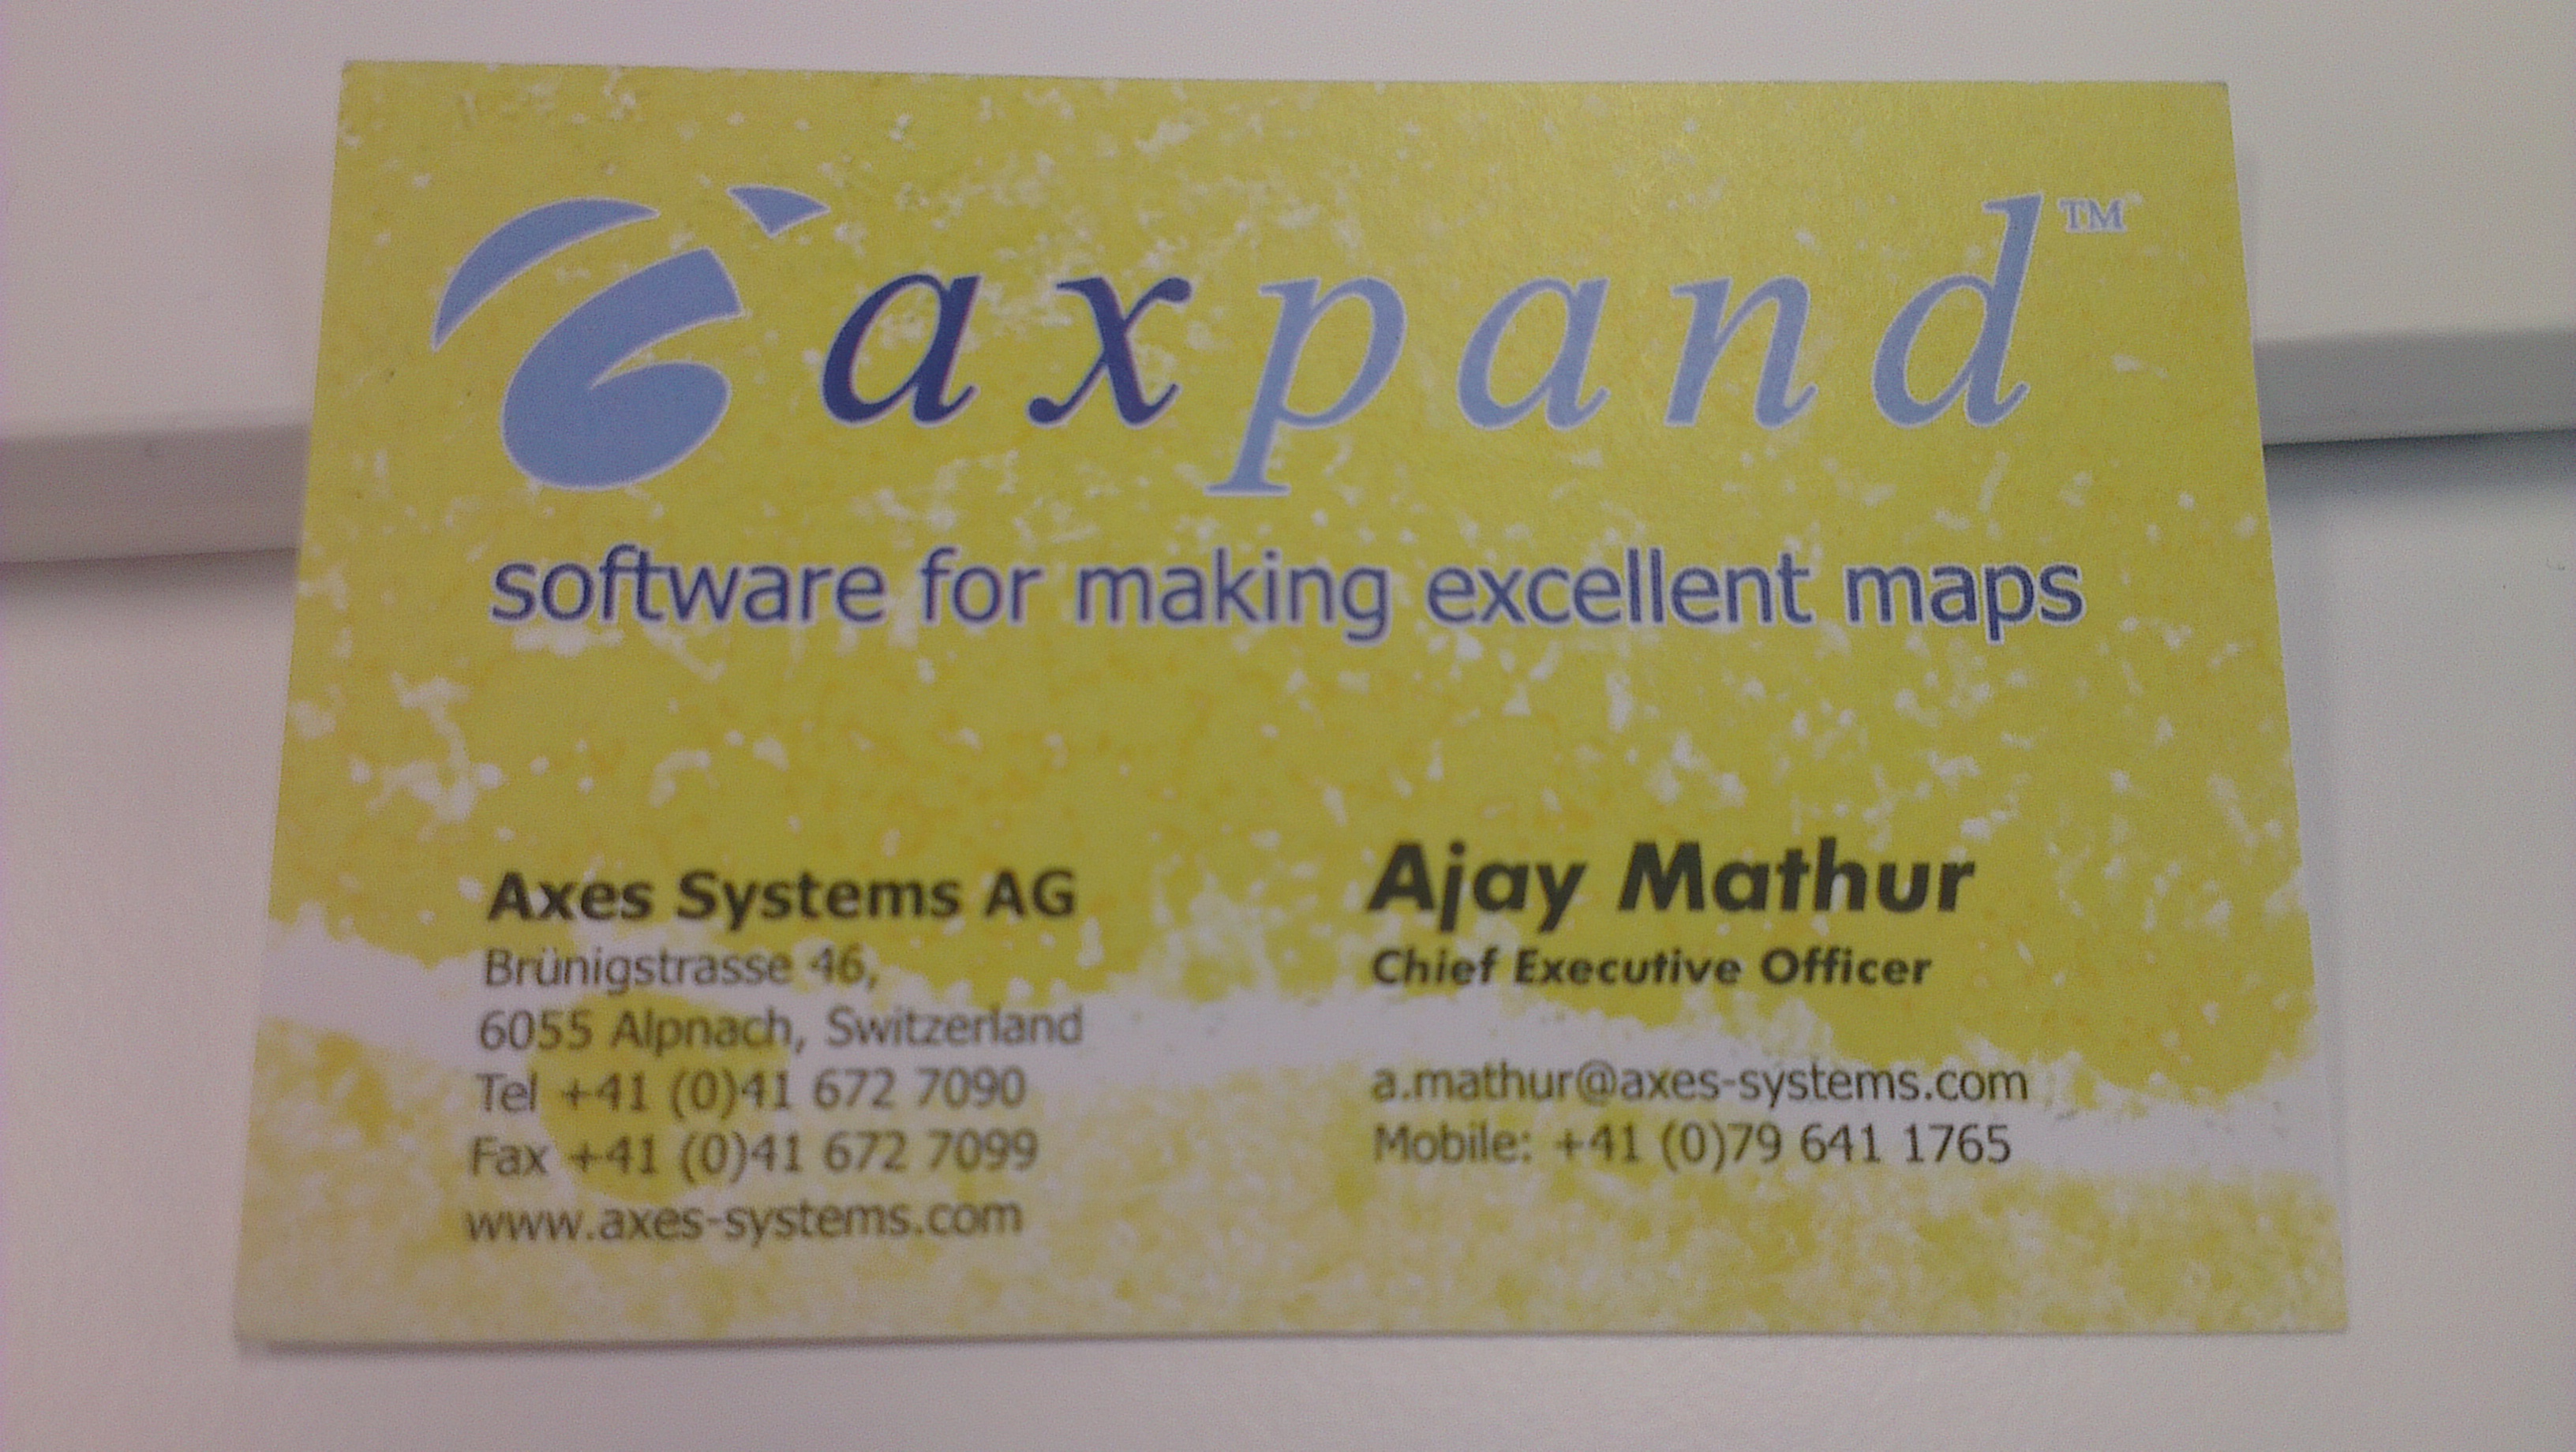
\includegraphics[scale= 0.06]{BlurredAMathur.jpg}
	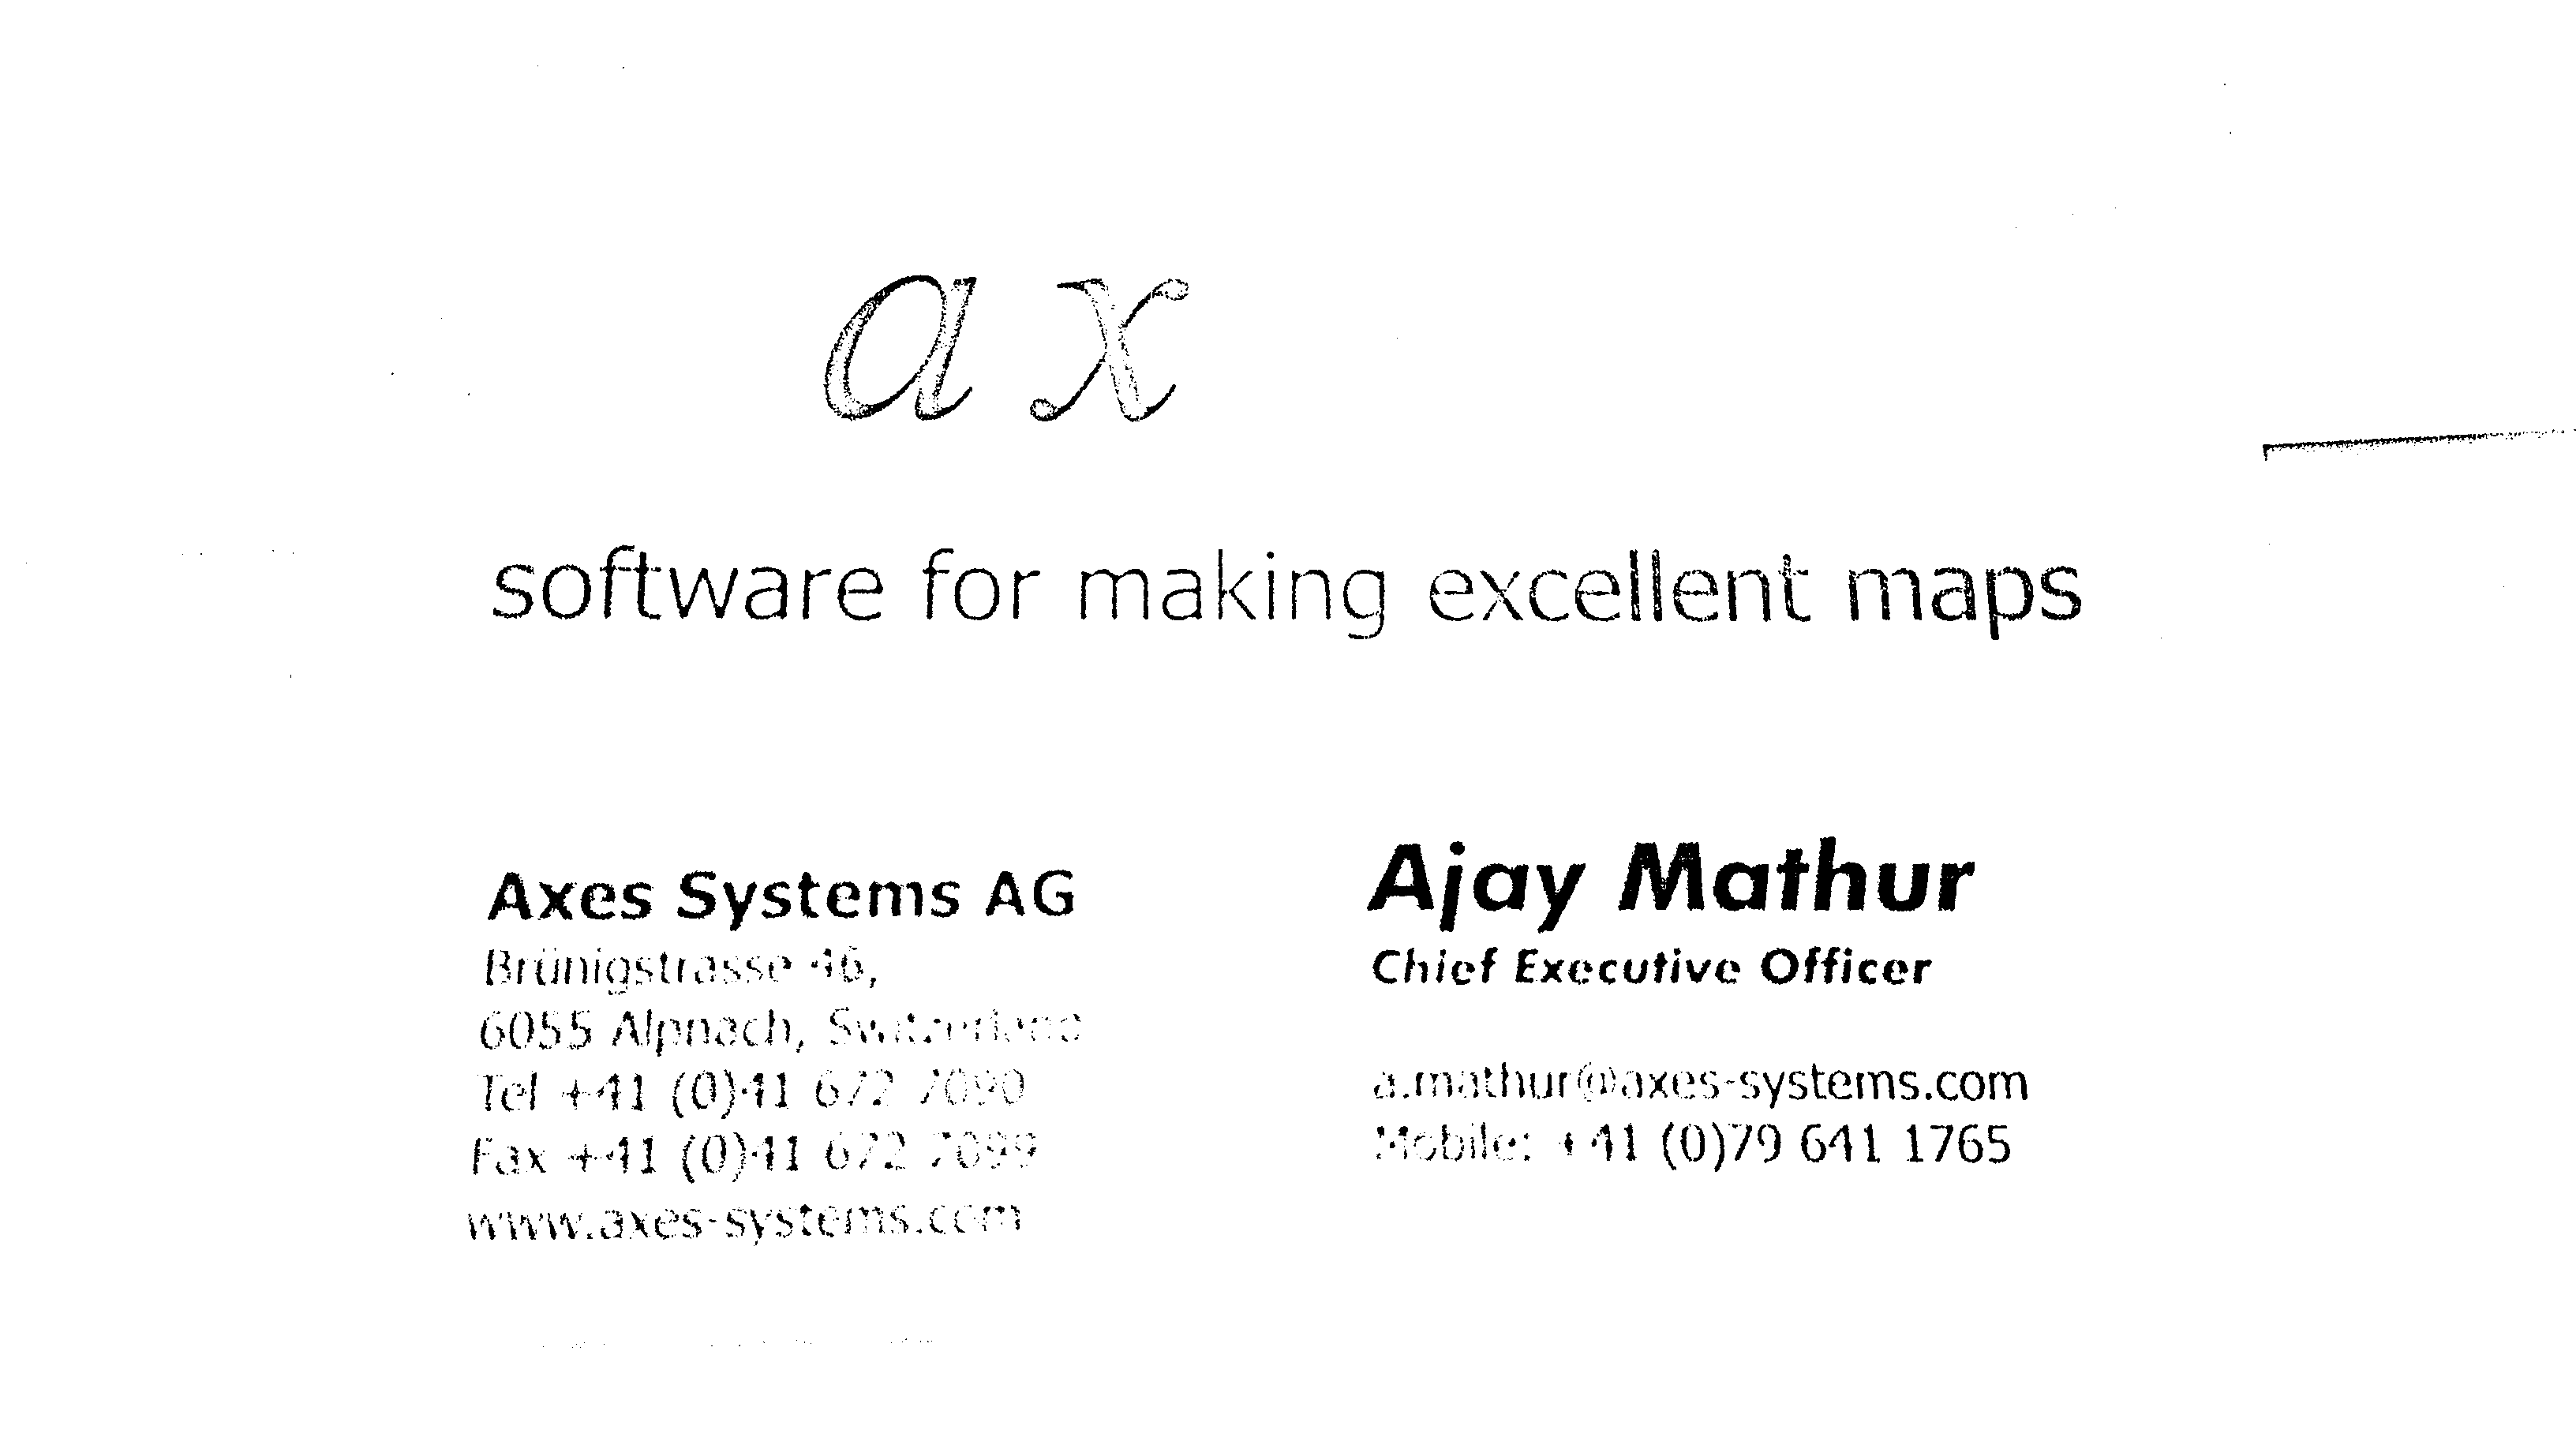
\includegraphics[scale= 0.06]{BlurredAMathurPhansalkar.png}
	\caption{ Die gleiche Visitenkarte unscharf fotographiert. Teile de Texts sind nicht mehr im Bild enthalten.}
\end{figure}
Auch wenn der Text nicht gänzlich fehlt so werden die Buchstaben nur Bruchhaft binarisiert, was zu einer sehr schlechten Texterkennung führt.
\begin{figure}[h!]
	\centering
	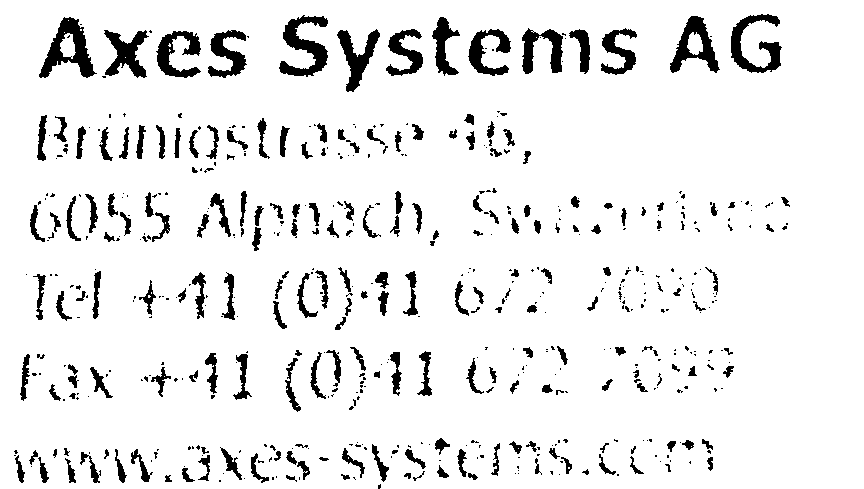
\includegraphics[scale= 0.3]{BlurredAMathurPhansalkarZoom.png}
	\caption{Ausschnitt des unscharfen Bildes zusammen mit dem von Tesseract erkannten Text.
	Der erkannte Text steht über den Boundingboxen geschrieben.}
\end{figure}

	

\section{Quellen}

\begin{enumerate}
\item \url{www.psprint.com/resources/powerful-business-card-fonts/} Aufgerufen am 20.12.2013
\item \url{absolutegraphix.co.uk/bestworstfonts.asp?strID=Guest} Aufgerufen am 20.12.2013
\end{enumerate}

\subsection{Tools und Applikationen}
%nomol en scheiss titel
\begin{enumerate}
\item \url{http://code.google.com/p/google-diff-match-patch/}
\end{enumerate}

\section{Anhang}


% Inhalt Ende 
\end{document} 